The previous section outlined the science case for a telescope on the lunar farside and the results are summarized in Appendix A.  Ideally, one would build a large and flexible observatory, and discussions for such telescopes are underway (e.g. \citealt{burns2021lunarfarsidelowradio}, \citealt{9438165}).  However, to take advantage of this unique opportunity for early measurements, two additional constraints inform the payload design: (1) land and operate before the end of the decade (by 2030) and (2) achieve the goals for a budget of US\$150M or less.  The design is therefore structured around these additional objectives, meaning it has similar schedule and budget requirements to missions under the NASA Commercial Lunar Payload Service (CLPS) program.  The lunar lander will have a diameter of approximately 4 m and a science payload mass of approximately 100 kg.  One main difference from the NASA CLPS program is our ability to work with potential vendors to increase compatibility between the lander and science payload. For example, the LuSEE-Night program carries its own power system (solar panel and battery) and communication system and requires the lander to electrically passivate itself at the end of the lunar day. This simplifies lander-payload interfaces and gives LuSEE-Night full control over the RFI environment at the expense of increased payload complexity, weight, and cost. For LFT3 we want to work much closer with the vendors and rely on lander for power and communication.   The primary concern is electromagnetic compatibility and the need to minimize radio frequency interference affects, which will be achieved by a combination of requirements on instrument design (syncing all clocks to precisely place power supply harmonics) and operational constraints (switching off non-essential equipment when taking science data). Table \ref{tab:constraints} summarizes the scope of the payload that fits within the constraints. These numbers represent an evolutionary and realistic step-up from the parameters of LuSEE-Night.

\begin{figure}
	\centering
	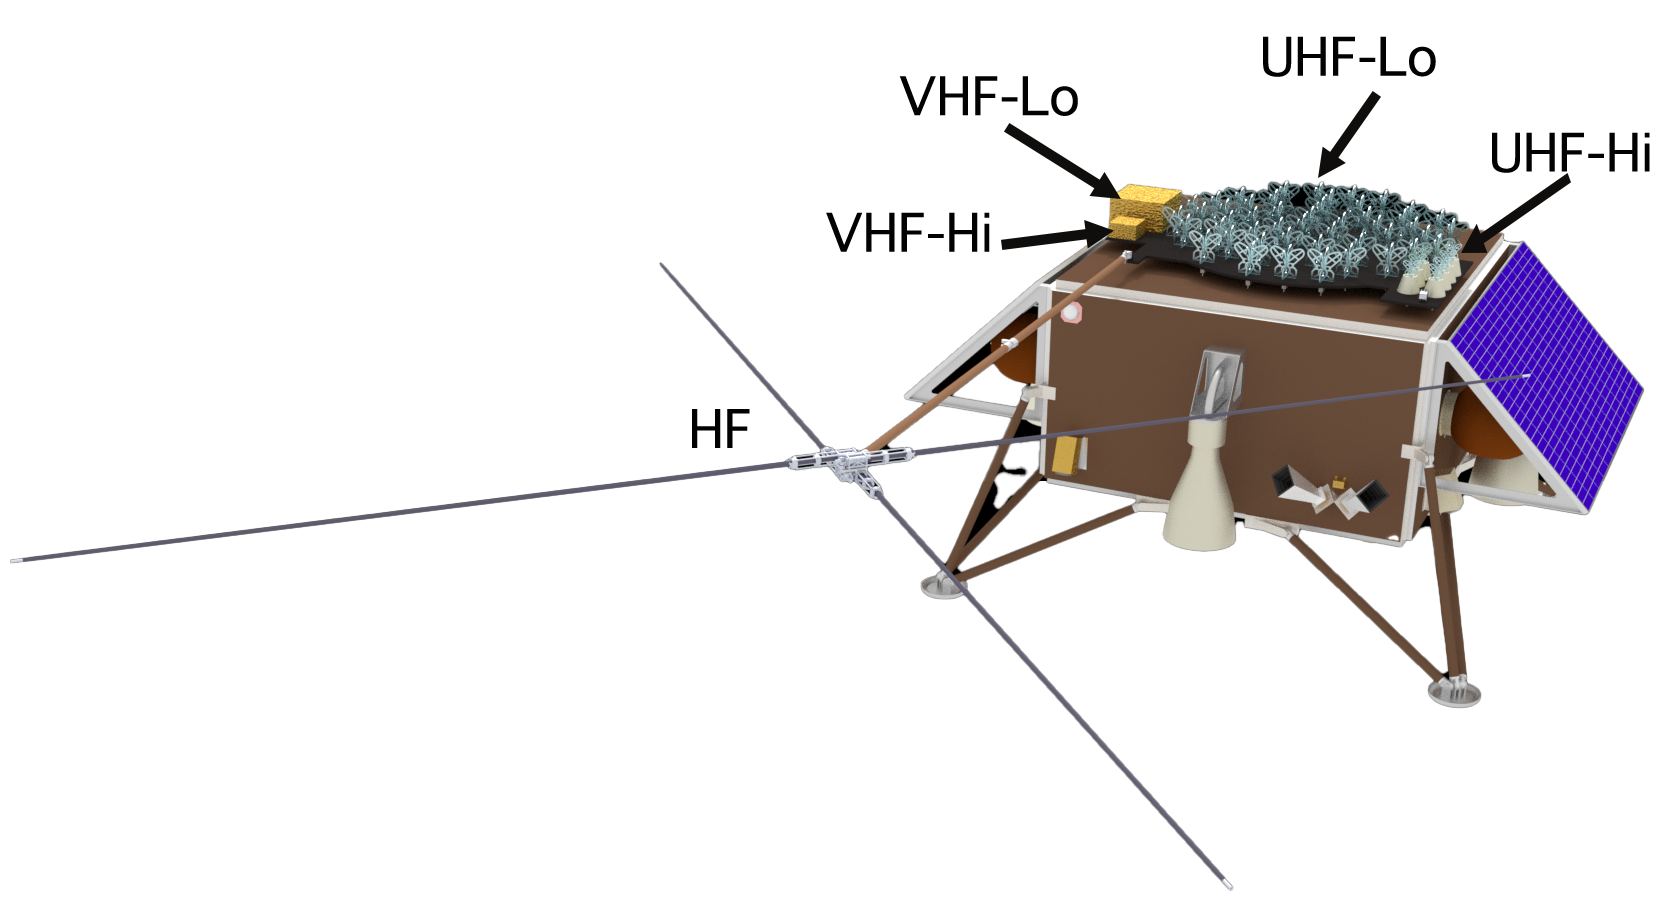
\includegraphics[width=\linewidth]{figures/LFT Deployed 02.png}
	\caption{Rendering of the generic science lander and payload.  The antennas are all located on the top deck, and the beamformer and processor are located in a thermal cavity directly below.  The antenna elements are annotated per band. \label{fig:render}}
\end{figure}

\begin{table}
    \caption{Payload Requirements}
    \begin{tabular}{|l|l|l|} \hline
    \textbf{Parameter} & \textbf{Value} & \textbf{Notes} \\ \hline
    \textbf{Span} & $\sim$4 m & This varies with vendor. \\ \hline
    \textbf{Mass} & 100 kg & This is the science payload mass. \\ \hline
    \textbf{Power (day)} & 200 W & Balancing day/night operations. \\ \hline
    \textbf{Power (night)} & 30 W & Included in the lander mass budget. \\ \hline
    \textbf{Comms} & 100 GB/month & The nominal budget includes 20 weeks of operation \\ \hline
    \textbf{Storage} & 20 TB & This coupled with comms and processing scopes the system. \\ \hline
    \end{tabular}
    \label{tab:constraints}
\end{table}


\begin{figure}
	\centering
	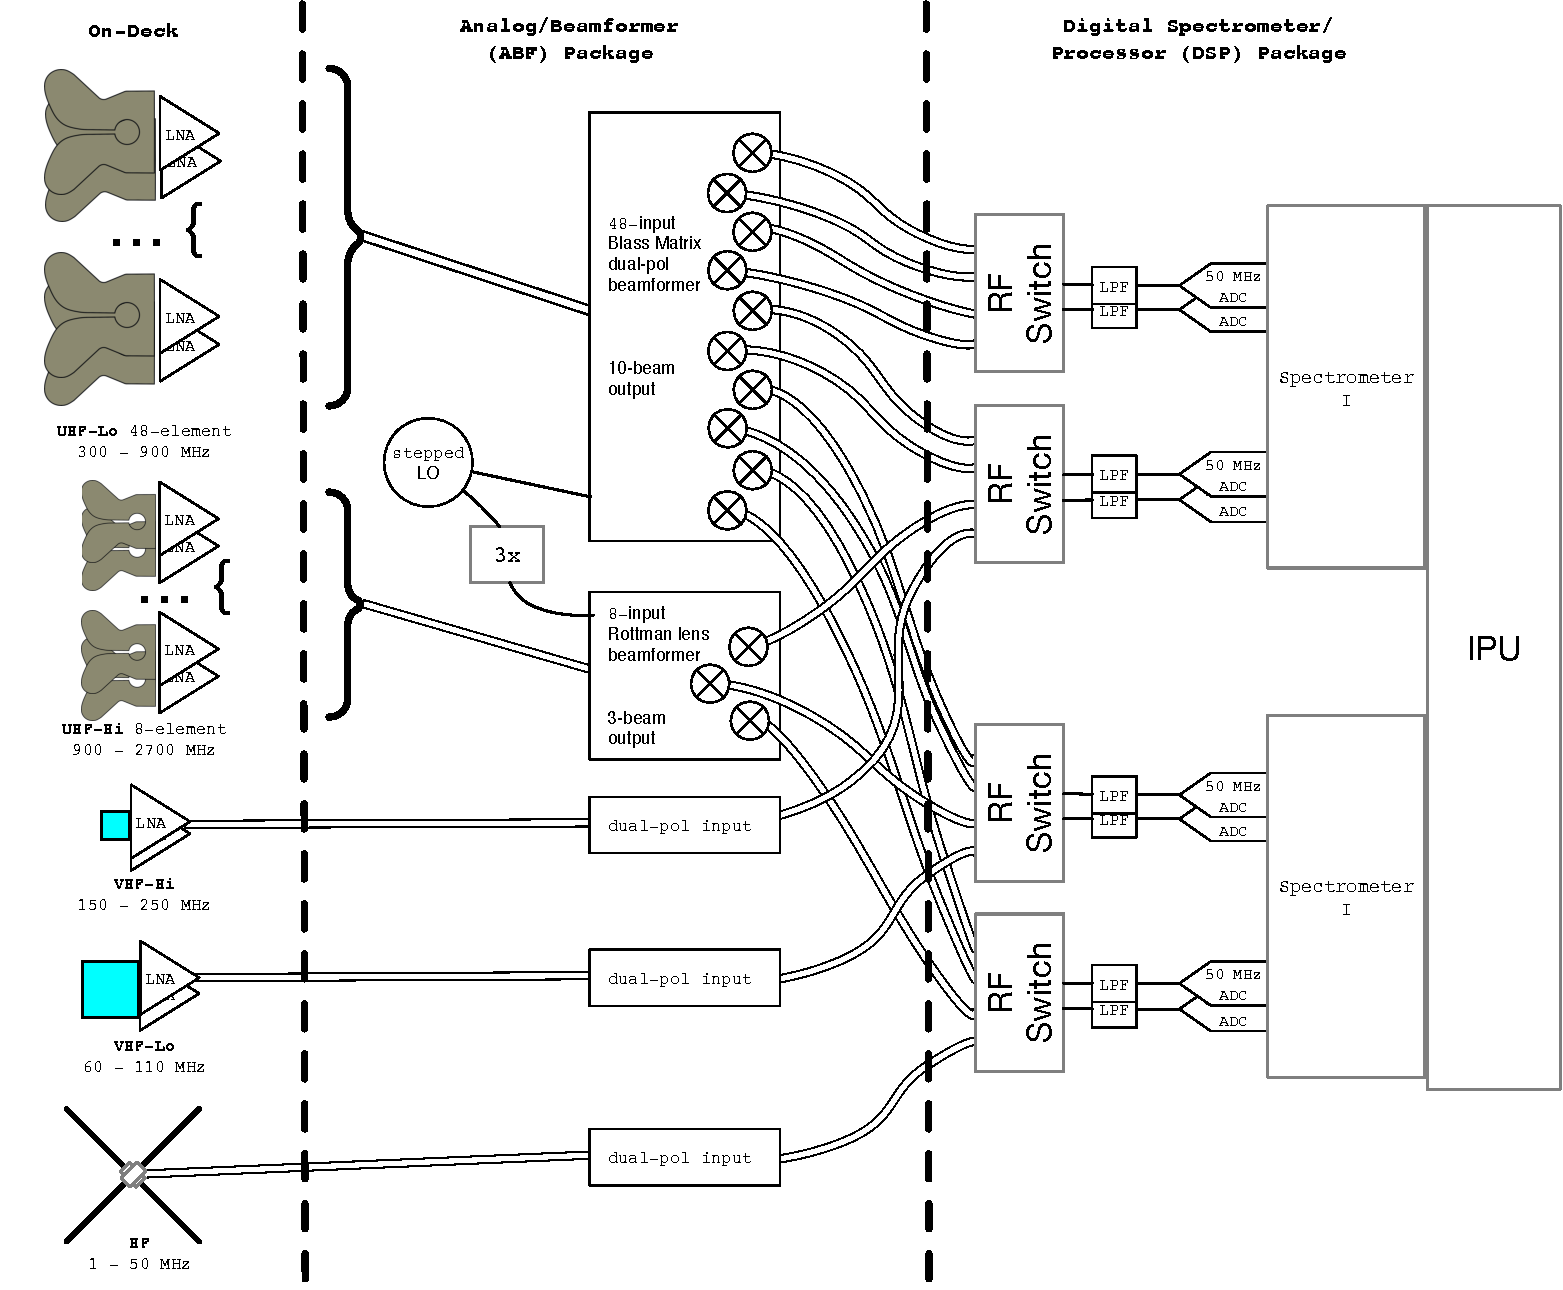
\includegraphics[width=\linewidth]{figures/SciencePayload.pdf}
	\caption{Block diagram of the science payload.  The five bands are shown on the left.  The UHF bands go into a heterodyne and beamforming system to chose the frequency sub-band and form the beams.  All of the RF inputs go into RF switches before digitization and processing.  The exact partitioning of the system will be addressed in the next design phase.  As currently shown, there are two spectrometers for redundancy.  The Instrument Processing Unit (IPU) conducts the processing and saves the data for transmission to Earth.\label{fig:block}}
\end{figure}


\begin{table}
    \centering
    \caption{Basic system parameters of the receiver sub-system.  The sensitivity is shown in Figure \ref{fig:freqbands}. There are a total of 16 sky-fixed dual-polarization beams, of which 8 can be observed at the same time subject to switching network constraints (see Figure \ref{fig:block}).}
    \label{tab:bandparam}
    \begin{tabular}{|l|l|l|l|l|l|} \hline
    \textbf{Band} & \textbf{Freq Range} & \textbf{Antenna design} & \textbf{Beams} & \textbf{Beam size (degrees)} \\ \hline
    \textbf{HF} & 1 - 50  &  Cross pseudo-dipole  & 1&  $45^\circ-90^\circ$ \\ \hline
    \textbf{VHF-Lo} & 60 - 110 & printed film &  1 & $80^\circ$ \\ \hline
    \textbf{VHF-Hi} & 150 - 250 & printed film & 1 & $80^\circ$  \\ \hline
    \textbf{UHF-Lo} & 300 - 900 & phased array (Vivaldi$\times$48) & 10 & $4^\circ-16^\circ$\\ \hline
    \textbf{UHF-Hi} & 900 - 2700 & phased array (Vivaldi$\times$8) & 3 & $20^\circ-60^\circ$ \\ \hline
    \end{tabular}
\end{table}

\begin{table}
\centering
\caption{Basic spectrometer parameters. LFT3 will operate two such spectrometers. \label{tab:spectrometer}}
\begin{tabular}{|l|l|} \hline
\textbf{Parameter} & Value  \\ \hline
Number of input channels & 8 \\ \hline
Bandwidth & $>$50\, MHz \\ \hline
Duty-cycle & 100\% \\ \hline
Correlation products & 4  \\ \hline
Spectral Channels & $2^{9}$ - $2^{22}$  (i.e. $512$ - 4$\times 10^6$ ) \\ \hline
Polyphase filterbank taps & 8 \\ \hline
ring-buffer size & 1\,second \\ \hline
Power-consumption & $<$12\,W \\ \hline
Additional capabilities &  technosignature search, pulsar signal detection \& folding, \\
& dedispersion, general transient detection\\ \hline
\end{tabular}
\end{table}


A rendering of the lander is shown in Figure \ref{fig:render} and a schematic of the science payload is shown in Figure \ref{fig:block}.
The five antenna subsystems are summarized in Table \ref{tab:bandparam}.  The UHF-Lo array covers most of the lander top surface with 48 dual-polarization wideband antenna elements. The array forms a fan of beams on the sky designed to cover 70\% of the lunar sky over time (Fig. \ref{fig:midband_beam_maps}). Formed beam output signals are downconverted and sampled in a 50 MHz subband that is scanned across the array operating bandwidth.  Efforts are underway to see if that bandwidth can be extended. The system design has two spectrometers whose preliminary specifications are shown in Table \ref{tab:spectrometer}. 




\begin{figure}
	\centering
	\includegraphics[width=\linewidth]{figures/midband_array_28cm_3dBSLL_beams_max.eps}
	\caption{Midband array formed beams over frequency. Scale is aperture efficiency in dB relative to a 3 meter diameter area. Beams are centered within 11 equal intervals over a 120 degree field of view.}
	\label{fig:midband_beam_maps}
\end{figure}

Operational constraints have a huge impact on the observation strategy, the derived data products, and the downloaded data.  The available full-day power is $\sim$200 W, which reduces to $\sim$30 W at night, and the expected download capacity is 100 GB/month.  The expected on-board memory will be 20 TB.  The beamformer and individual antennas will produce dual-linear polarizations.  The spectrometer will produce pseudo-Stokes dynamic spectra of varying spectral/temporal resolutions. On an appropriate trigger, it will also produce full base-band data over the last trigger. 
The on-board instrument processor unit (IPU) will provide any post-processing of the dynamic spectra and coordinate memory and transmission back to Earth.  The communication back to Earth for data will be limited to the lunar day.  The concept of operations is discussed in Section \ref{sec:conops}.

\subsection{Lunar Farside Location}
The lunar farside is a unique location in the solar system in that it is the only area that never faces Earth due to tidal locking.  This means that it is always blocked from terrestrial and near-terrestrial radio frequency transmissions.  This importance was recognized in the 1970s when the International Telecommunication Union (ITU\footnote{The ITU is the international organization that handles electromagnetic emission across national boundaries.} defined the Shielded Zone of the Moon (SZM) as “compris[ing] the area of the Moon’s surface and an adjacent volume of space which are shielded from emissions originating within a distance of 100,000 km from the center of the Earth” \citep{itu_rr_2024}.  This essential radio quietness will be exploited by LFT3.  Figure \ref{fig:orbit_banana} shows a projection of the lunar orbit to give a sense of scale of Earth's size, the Moon's size, the distance from Earth, and the variability of the orbit.

\begin{figure}
	\centering
	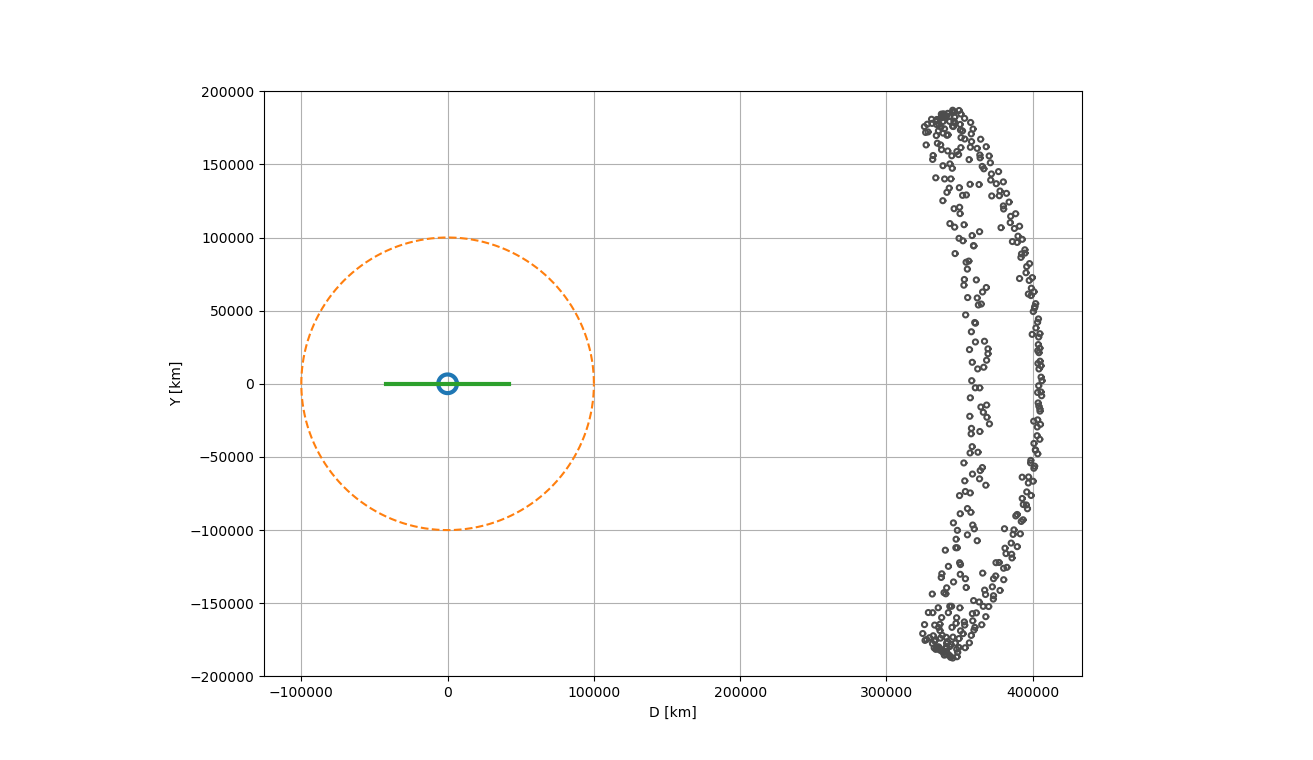
\includegraphics[width=\linewidth]{figures/lunar_orbit_dist}
	\caption{Projection of the lunar orbit showing the relative sizes and variability. The Earth is at the origin and the location of the Moon is shown for every day of 2028. The x-axis is the distance from the Earth and the y-axis is the distance out of the equatorial plane.  The green line is the geostationary arc and the orange circle is the 100,000km SZM defining circle.  The relative sizes of the Earth and Moon are to scale.}
    \label{fig:orbit_banana}
\end{figure}

The landing site coordinates of 23.78930°S, 182.13737°E (Fig. \ref{fig:landing_site}) are well within the SZM and are also near the LuSEE-Night landing location, with which it will coordinate.  In the Equatorial Farside region, lunar days and lunar nights each last approximately 14 Earth days. This results in survival temperatures ranging from 100 K to 400 K \citep{2012JGRE..117.0H18V}.  Additionally, landing near LuSEE-Night provides a known location with recent landing experience, increasing the chance of a successful landing.

\begin{figure}
	\centering
	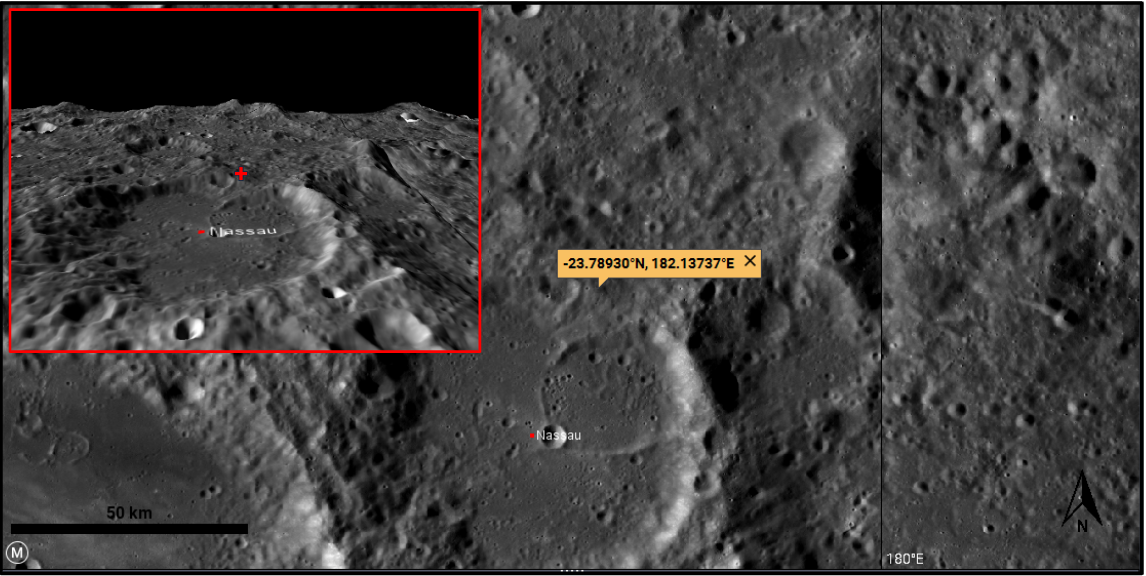
\includegraphics[width=\linewidth]{figures/Landing site overview.PNG}
	\caption{LFT3 Farside Landing Site - Micro View JMARS}
    \label{fig:landing_site}
\end{figure}

\subsection{Concept of Operations}
\label{sec:conops}
In this section, we outline the LFT3 science operations framework designed to efficiently support the proposed science goals by allocating appropriate mission resources ----such as observation time and downlink capacity---to each science objective. A more complete description can be found in \cite{prabu2025lft3}. The science goals described in this white paper are broadly grouped into three categories which correspond to the categories in Table \ref{tab:scisum}: lunar-exclusive science goals, lunar-augumented science goals, and proof-of-concept science goals. Lunar-exclusive science goals include measurements uniquely enabled by the radio-quiet, ionosphere-free environment of the lunar farside---such as unambigious searches for technosignatures, detection of low DM transients, cosmology, and legacy RF surveys of the Moon's farside that will serve as a baseline before future RFI contamination. Lunar-augumented science goals build upon and enhance Earth-based observations with additional complementary low-frequency wideband measurements, thus improving the overall scientific understanding of known astrophysical sources. Proof-of-concept science involves replicating measurements that can also be performed from Earth, with the goal of validating LFT3's scientific capabilities and calibrating its measurements against the ones from Earth-based observatories. Examples of this will be observing bright quasars, pulsars, and hydroxyl masers. A high-level categorization of all science goals into these three groups is shown in Figure \ref{fig:sciencegoals}.


\begin{figure}
	\centering
	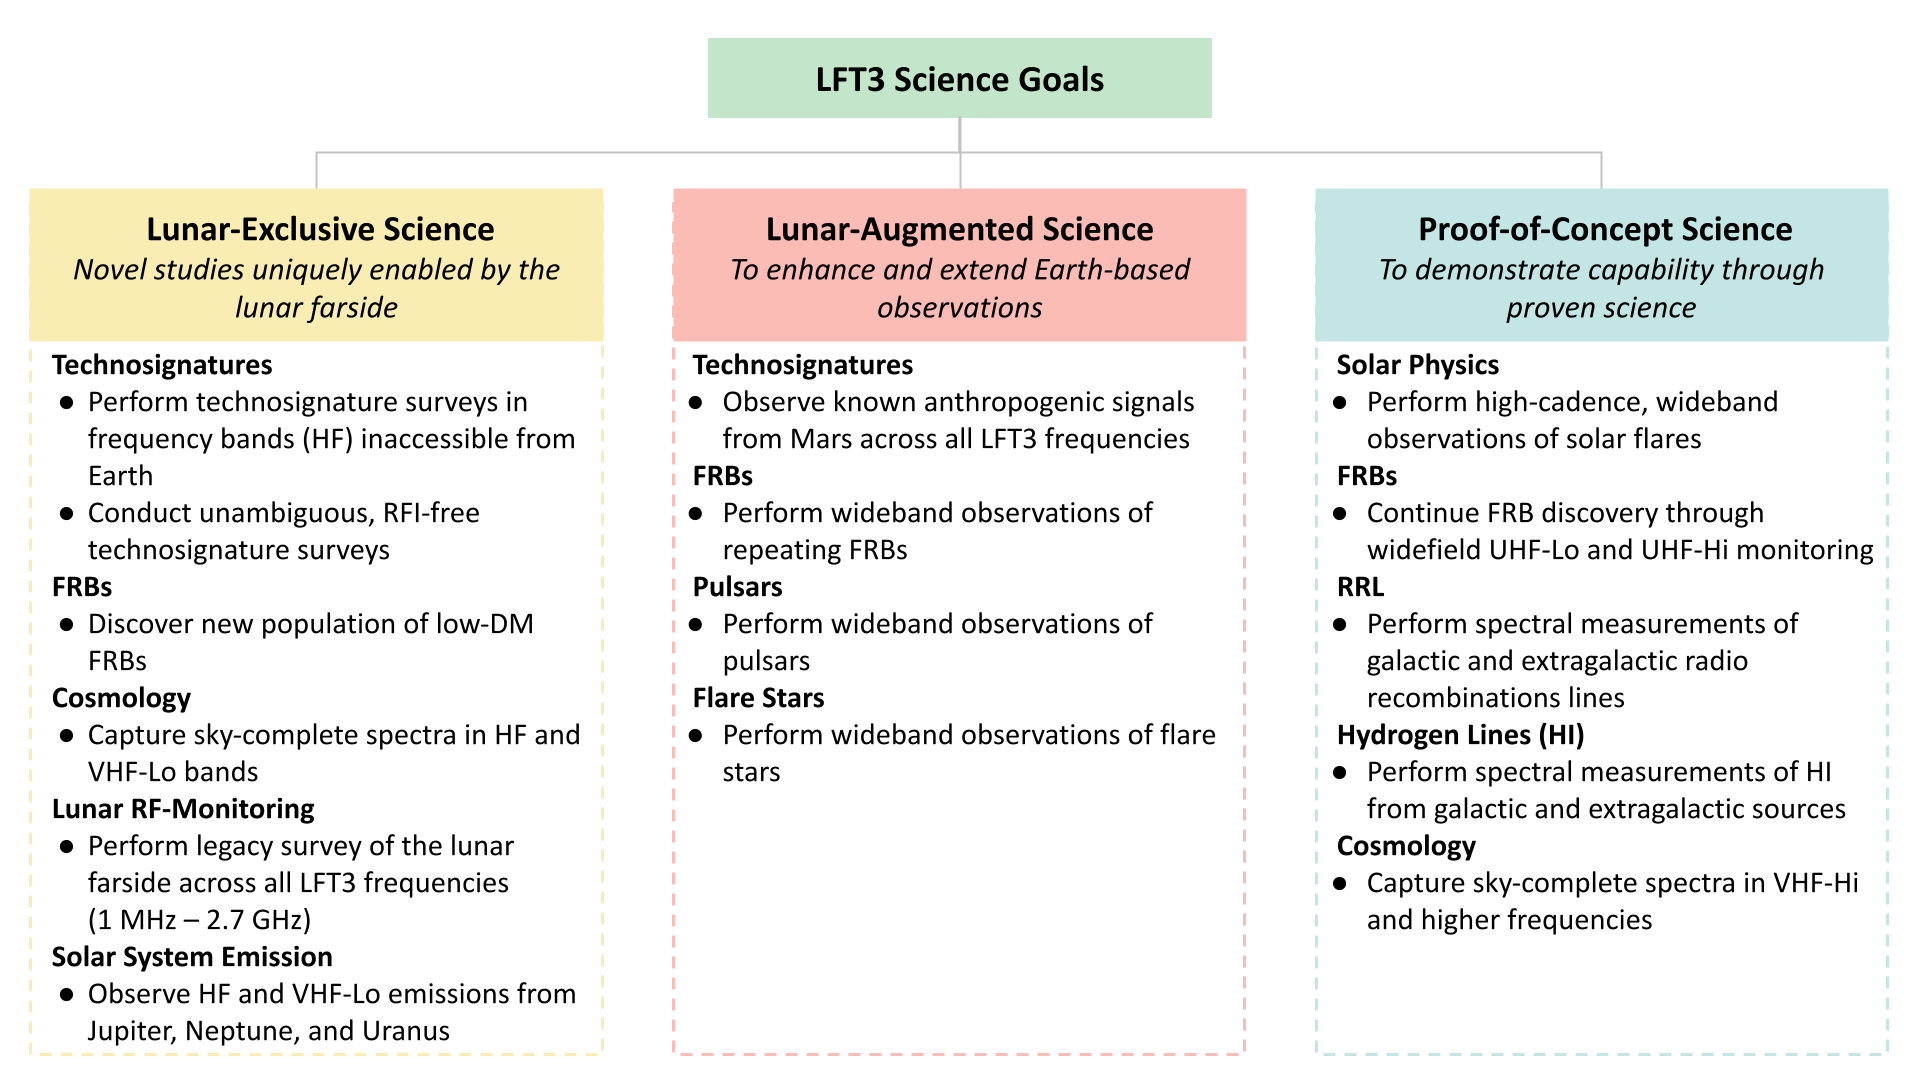
\includegraphics[width=\linewidth]{figures/LFT3ScienceGoals2.png}
	\caption{A high level breakdown of LFT3 science goals into lunar-exclusive science goals, lunar-augumented science goals, and proof-of-concept science goals (image borrowed from \cite{prabu2025lft3}.)}
	\label{fig:sciencegoals}
\end{figure}

All LFT3 science operations will be conducted in two distinct modes: real-time observations and targeted observations. A real-time processing pipeline will operate continuously across all observed fields, constantly looking for transients and technosignature candidates. A real-time search system that runs throughout the 20-week mission life of LFT3 maximizes our likelihood of serendipitous discoveries of transient events. Due to their persistence in the sky, all other science targets (such as pulsars, Sun, solar system planets, etc.) will be observed as the targeted observations with appropriate scheduling (such as choice of beam to process, time and frequency resolution of the output science data, frequency tuning, and number of Stokes parameters to record) as and when the target appears within LFT3's visible sky. A complete breakdown of the observing schedule for these science targets and the corresponding generated science data volume can be found in \cite{prabu2025lft3}.

Due to the lack of a line-of-sight link to LFT3 from Earth-based groundstations, science data products from LFT3 must be relayed to Earth through an intermediate lunar orbiting satellite. Currently, this method of downlinking data back to Earth is effectively limited to 100 GB/month. Hence, to ensure optimal use of this limited data rate, we define four different science data products that will be produced by LFT3, namely, baseband data, sky-complete spectra, high-resolution dynamic spectra and event catalog (see Table \ref{tab:data}). For high SNR transient and technosignature events seen by LFT3, 1s of baseband data (about 2GB/s) will be downlinked back to Earth. For all other targeted science observations, only high-resolution dynamic spectra (produced at a rate of $0.0004 - 50$ MB/s based on the science target being observed) are transmitted back to Earth from the LFT3 beam containing the target, and the time/frequency resolution of these dynamic spectra is dictated by the science requirements of the target. For all the fields being observed by LFT3 during its life, a coarse resolution spectra (1MHz frequency resolution and 5 minute time integrations) called the sky complete spectra are generated. This sky complete spectra maps out the complete celestial sphere seen by LFT3 during its life, and contributes towards the comology and lunar-RF monitoring studies proposed in this white paper. The payload also maintains an onboard catalog of low-SNR pulse signals in the form of an event catalog, which will be used for gathering statistics of false positives (and any underlying low-SNR astrophysical transient population) seen by the instrument.

\begin{table}
    \centering
    \caption{Uncompressed volume of data products produced by LFT3 per lunar cycle (28 Earth days). Note that the total data generated is over the 100GB limit. The science data can be fit within the budget using data compression methods, which may potentially be lossy.}
    \begin{tabular}{|l|l|l|l|} \hline
    \textbf{Product type} & \textbf{Data Volume [GB]} & \textbf{Total integration time} \\ \hline
    Baseband data        & 20 &  10 \, seconds \\ \hline
    Dynamic spectra      & 255.6 & 336\, hours  \\ \hline
    Sky-complete spectra & 0.5 & 672\, hours \\  \hline
    Event Catalog        & $\le$ 1 & $1.4\times 10^9$ events (at 5$\sigma$) \\ \hline
    Meta-data and housekeeping & $\le 1$ & - \\ \hline
    \end{tabular}
    \label{tab:data}
\end{table}

Overall, the mission timeline aims to launch the LFT3 payload in 2028, with a high-level functional requirement for 20 weeks of operation. The high-level science traceability matrix of the mission can be found in Figure \ref{fig:STM}. The proposed science operations plan in \cite{prabu2025lft3}, aims to meet all mission objectives within the 20-week time frame, by allocating sufficient observation times to each of the science goals and a data management plan to download the highest priority data.
